\clearpage\section{系統設計與實作}

\subsection{系統架構}

\subsubsection{研究問題與功能分支}
既有系統由協調者（Coordinator）掌管任務、資料邊界與記憶權限；中立報告鎖定之後，才分流到各個決策機制。網頁、命令列與程式介面共用同一套流程，目的是讓執行與稽核的結果一致。對應到研究架構：模型路由器（Model Router）對應 RQ2 的模型組合；領域辯論模組（Domain Debate Module）與最終整合者（Final Aggregator）對應 RQ3 的領域推理與上層整合。各模組的實作狀態整理於表~\ref{tab:modules}，狀態更新截至 2026 年 10 月 15 日。RQ1 模組已用於 180 案；RQ2／RQ3 的核心程式已有原型與合成測試，但不代表真實模型資格檢驗、完整必要對照或正式實驗已完成。

\subsection{功能模組}

\begin{table}[H]
\centering\small
\caption{功能模組的實作狀態}
\label{tab:modules}
\begin{tabularx}{\textwidth}{@{}L{.30} L{.20} Y@{}}
\toprule
模組 & 狀態 & 對應 \\
\midrule
協調者與資料快照 & 已實作 & RQ1 使用 \\
研究代理人 & 已實作 & RQ1 使用 \\
短期與長期記憶 & 已實作 & C、D 的裁決者可讀 \\
裁決者、守門員與回測 & 已實作 & RQ1 使用 \\
模型路由器 & 已實作原型 & RQ2；已隔離條件記憶，真實模型資格待補 \\
領域辯論模組 & 已實作原型 & RQ3；必要對照已有合成驗證，真實資格待補 \\
最終整合者 & 已實作原型 & RQ3；輸入含引用證據與基準率 \\
\bottomrule
\end{tabularx}
\end{table}

\subsubsection{協調者與資料快照【已實作】}
協調者負責固定案例、實驗規則、截止時間與模型設定；資料代理人負責建立不可更動的資料快照，快照的雜湊值與證據編號會連到執行紀錄。

\subsubsection{研究代理人【已實作】}
四個面向的研究代理人，各自在同一個時間邊界內摘要並引用證據，產生鎖定的中立報告與各領域的輸出；驗證失敗而改用來源原文摘錄的降級處理時，系統也會記錄。

\subsubsection{短期記憶與長期記憶【已實作】}
\frlabel{sec:memory}
短期紀錄保存每次呼叫的提示詞指紋碼、隨機種子、用量、辯論內容與裁決；長期記憶只讀分析日以前已到期的同一檔股票案例。目前 C、D 的裁決者可以讀長期記憶，A、B 不行，所以解讀補充比較時要把這個權限差異考慮進去。此外，記憶必須「到期」才能被讀取，以避免過去的案例讀到未來的結果。

\subsubsection{裁決者、守門員與回測【已實作】}
裁決者逐項核對論點與證據後，輸出候選方向；守門員檢查引用、資料覆蓋、波動度與基準率歷史，必要時降級。回測用相同的開盤進出場、成本與日序列計算，不會把四個領域的看法當成四個部位。

\subsubsection{模型路由器【已實作原型，尚無正式結果】}
模型路由器目前實作的核心功能是：記錄每個代理人的身分、起始立場、每輪立場與模型編號／版本，並依 M1/M2 的平衡配置（配置 X、Y）呼叫不同的模型；第二輪只改立場，引用的對象仍是同一個代理人的第一輪。系統禁止在背景默默換成別的模型（fallback），也要記錄 API 是否支援固定種子，以及服務商端是否有模型版本漂移。

\subsubsection{領域辯論模組【已實作原型，尚無正式結果】}
領域辯論模組目前實作的核心功能是：把同一份快照中各領域的證據，分給各領域的看多／看空，依指定的辯論規則執行，並保存各領域的辯論逐字稿與領域看法。證據的命名空間與可讀取的權限都要驗證。

\subsubsection{最終整合者【已實作原型，尚無正式結果】}
最終整合者目前實作的核心功能是：讀取格式統一的四份領域看法、其引用證據與基準率，評估其中的衝突、反面證據與資料缺口，輸出一個最終候選決策；它的提示詞、輸入順序與記憶都要版本化，之後仍然交給相同的守門員。

\subsection{介面設計}

\subsubsection{研究台與流程追蹤}
介面設計有兩個原則：「流程看得見」與「步驟有引導」。頁面上方的資料流向圖（圖~\ref{fig:ui}）會即時顯示每個案例，從資料來源、研究代理人、中立報告、四組決策，到風控與回測的進度；點選任何一個節點，就能看到該步驟的輸入、模型輸出與紀錄。下方依「資料準備、建立實驗、代理人執行、統計結果」四個步驟分頁，使用者可以依序完成一次完整的實驗，同時查看執行終端與工作佇列。

\begin{figure}[H]
\centering
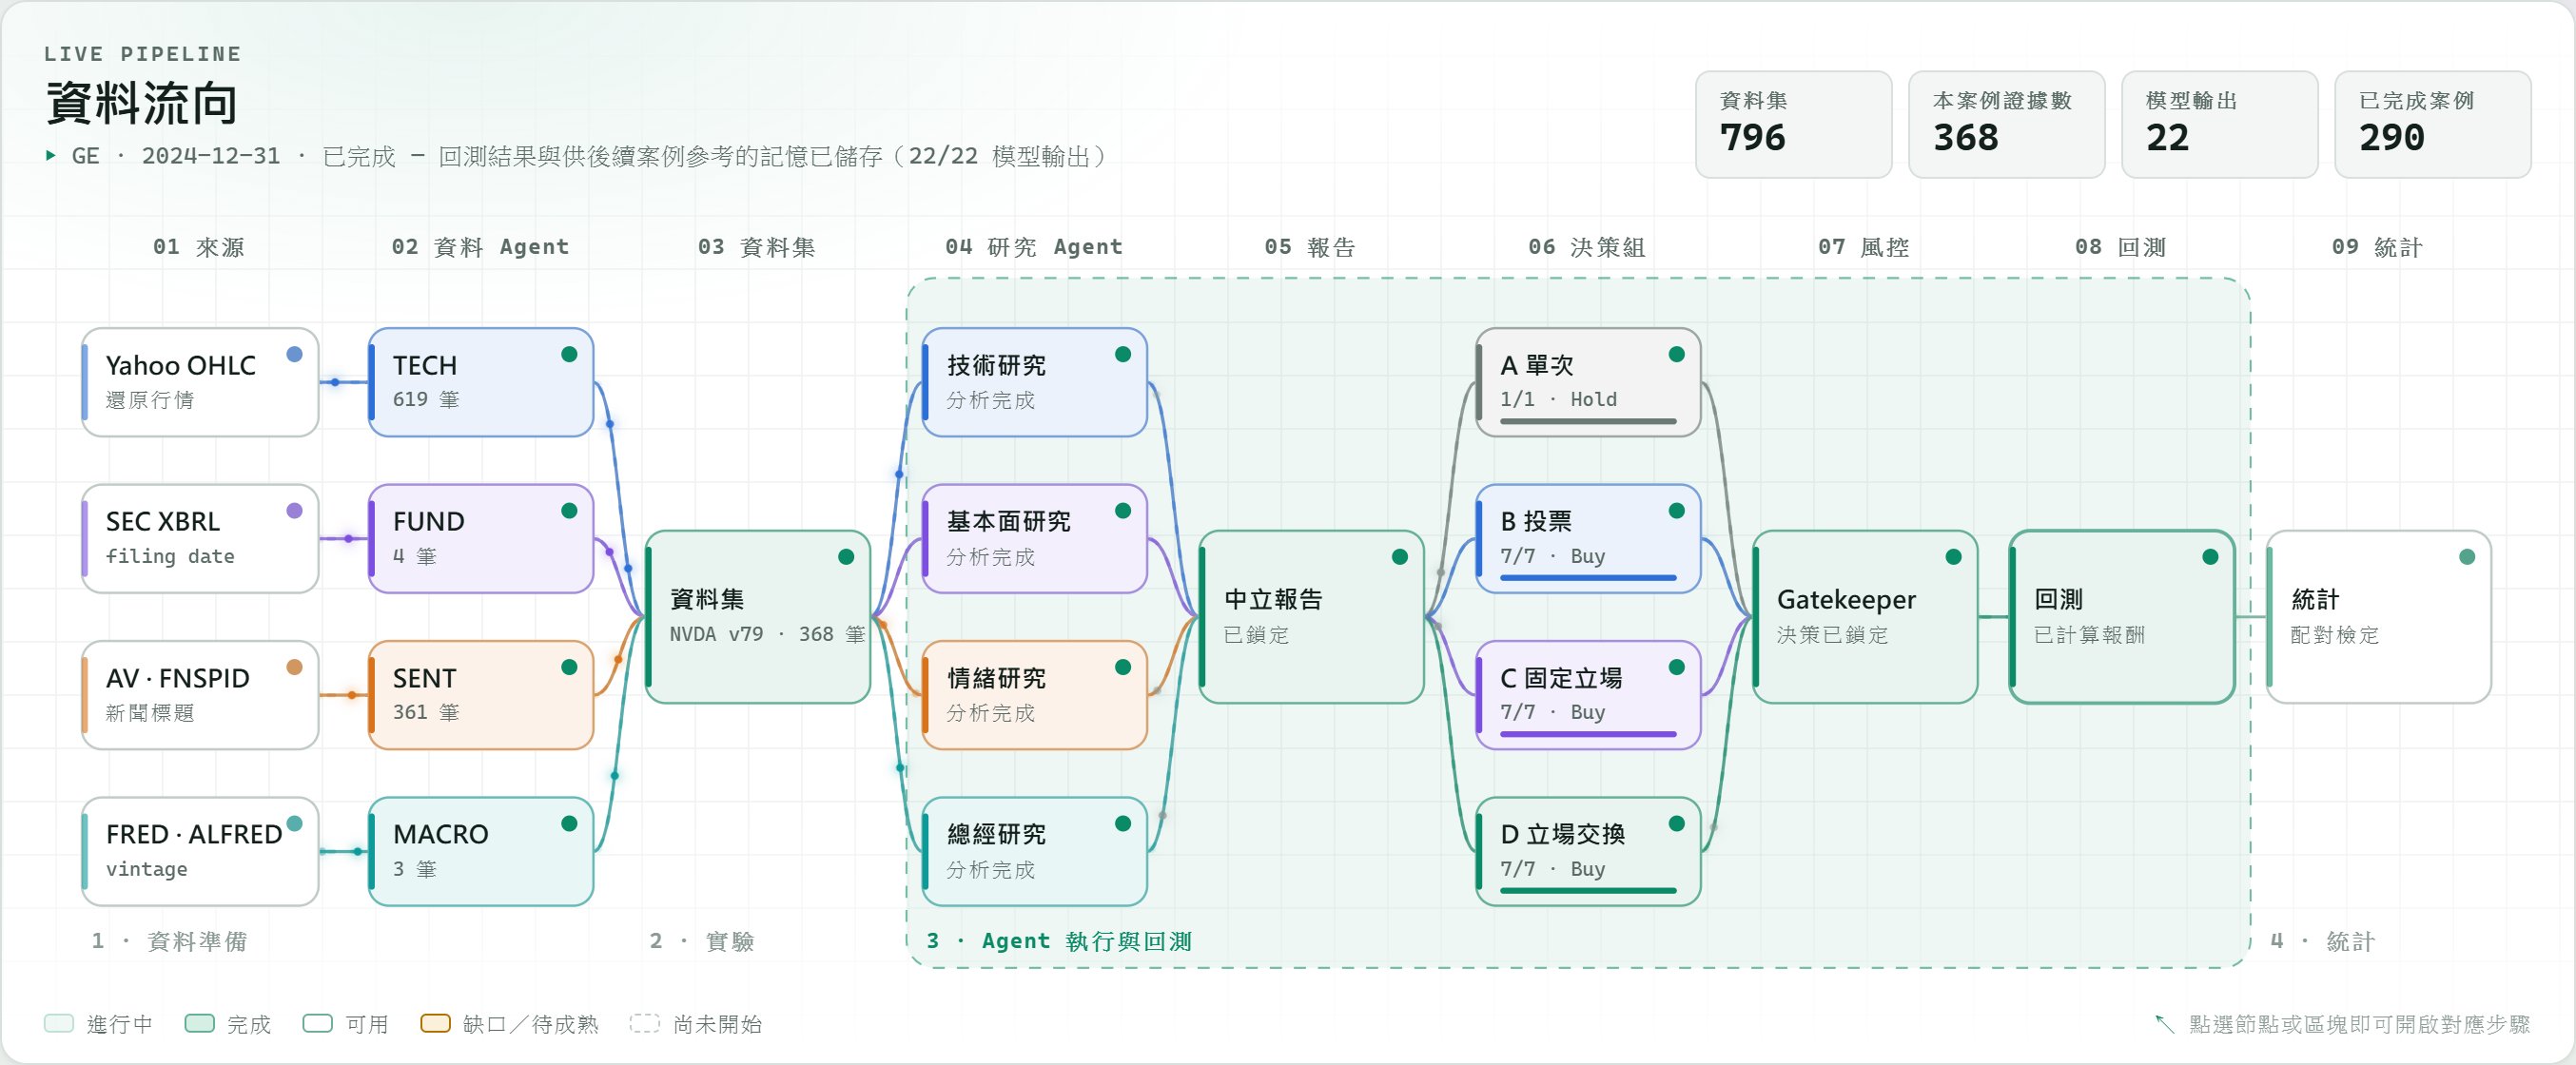
\includegraphics[width=\textwidth]{figures/ui-pipeline.png}
\caption{網頁介面的資料流向圖（一個已完成的案例）。由左至右依序為資料來源、資料代理人、資料快照、研究代理人、中立報告、四組決策、守門員、回測與統計。}
\label{fig:ui}
\end{figure}


介面以執行狀態與來源追蹤來支援研究檢查；模型的指派、論證、裁決與資源使用的紀錄，都應該能對應到單一案例。

\subsection{實作流程與驗證}

\subsubsection{開發流程}
系統依「資料、研究、決策、回測、統計」的順序逐步開發。每完成一個模組，先用模擬資料與小樣本測試，再用少量真實案例試跑，最後才進行正式實驗。開發過程中主要的挑戰與對策如下：

\begin{itemize}
  \item 時間邊界：財報與新聞要依「何時才看得到」篩選，避免分析日之後的資訊混進輸入；總經資料改用歷史版本，排除事後修正的影響。
  \item 模型輸出不穩定：模型常引用不存在的證據或輸出格式錯誤，所以用結構化輸出、證據短代稱與自動重試處理；模型也常自己改寫數字，所以改成要求用證據代稱來指稱事實。
  \item 結果可重現：系統設計上，在事前登記時鎖定程式與模型版本，每一步推理前後都核對模型權重，版本不符就拒絕執行。實際執行中仍有未完整保存的項目（FinBERT 版本、Gemini 呼叫設定、行情調整版本），見\frref{sec:repro}。
  \item 長時間執行：網路中斷時自動暫停，恢復後接著跑，已完成的步驟不重做，目的是讓 180 個案例在一致的條件下完成；180 案的原始輸出與版本對應，仍須在定稿前補齊。
\end{itemize}
\subsubsection{稽核紀錄與版本核對}
系統設計要求模型輸出在寫入前先驗證，並為每次呼叫建立稽核紀錄。下列項目是系統所支援的紀錄內容；現有 180 案是否全部具備完整紀錄，仍須以最終匯出清單逐案核對：

\begin{itemize}
  \item 提示詞中的證據用短代稱（E1、E2、$\ldots$）呈現，模型回答後再由程式對應回真正的識別碼。這樣可以避免模型抄錯很長的識別碼，也避免識別碼裡的申報編號洩漏公司身分。
  \item 引用的證據必須存在；如果引用不存在的證據或格式錯誤，系統會用明確的訊息要求重試，最多三次。
  \item 數字檢查：新版要求代理人用證據代稱指稱事實，而不是重述數字。敘述中如果還是出現沒有任何證據數值支持的數字（期間名稱、日期、來源值的四捨五入或截位不算），只記錄下來並依組別報告比例，不重試，也不修改文字。
  \item 凍結與身分核對：每一步推理前後，都核對模型權重的指紋碼；取不到時就暫停，之後可以接續執行；如果確認前後不同，該案例就永久作廢。程式原始碼的雜湊值也納入實驗規則的雜湊值，只要程式被改動就拒絕續跑。連線故障連續發生時，會暫停派發新案例，停滯太久時自動關閉 GPU 主機。
  \item 系統支援逐案匯出實驗規則設定、中立報告、證據登錄、執行軌跡、記憶、決策、逐案例回測、彙總指標與辯論逐字稿；本文不以此功能宣稱現有 180 案已全部完成可重現性核對。
\end{itemize}
\subsection{實作上的挑戰}

\subsubsection{格式不同與輸入長度限制}
不同模型的結構化輸出格式、分詞方式（tokenizer）與可讀的內容長度各不相同。轉接程式不能偷偷加入額外的金融資訊，也不能默默截掉某一方的反面證據。所以需要統一輸出格式、保存模型的原始回應與截斷紀錄，限制輸入長度並記錄失敗的情況。

\subsubsection{資源公平與領域輸出標準化}
呼叫次數相同，不代表 token 用量、成本或延遲相同；四個領域平行執行時，實際花費的時間與累計的推理時間也會不一樣。各領域看法的長度、缺漏值、證據與反面證據欄位如何標準化，會影響上層的裁決，因此格式與提示詞必須先鎖定，不能看完績效再調整權重。

\subsubsection{模型能力造成的混淆}
有了模型路由，並不表示就能識別出「異質性」本身的效果。模型能力的組合、裁決者對某種文風的偏好，以及不同模型的訓練記憶風險，都可能影響比較結果，所以要靠分開設定模型條件、控制輸入內容，並限定結果的適用範圍來解讀。

\clearpage\section{結果與討論}
\subsection{既有實驗規則下的機制比較}
本節呈現 qwen3:32b、季度實驗規則 v3-1002.3 下的既有回溯比較，以及同一批案例的 Gemini 探索性分析。結果只適用於這個模型、這套流程與這批資料；本節不能當成「不同模型辯論」或「領域專業化架構」的績效證據。


\subsubsection{qwen3:32b 的績效與配對檢定}
180 個案例（季度實驗規則 v3-1002.3）全部完成，沒有排除任何案例。表~\ref{tab:main} 是四組的績效，表~\ref{tab:tests} 是配對檢定。

\begin{table}[H]
\centering\small
\caption{四組績效（180 案，60 個交易日，已扣除交易成本）}
\label{tab:main}
\setlength{\tabcolsep}{5pt}
\begin{tabular}{@{}lccccc@{}}
\toprule
組別 & 出手率 & 條件準確率 & 累積報酬 & 最大回撤 & 年化 Sharpe \\
\midrule
\grp{A}\ 單次判斷 & 78.3\% & 56.0\% & 1.85\% & $-1.81\%$ & 0.44 \\
\grp{B}\ 獨立投票 & 79.4\% & 55.9\% & 1.95\% & $-1.83\%$ & 0.46 \\
\grp{C}\ 固定立場辯論 & 100\% & 58.3\% & 2.51\% & $-1.47\%$ & 0.59 \\
\grp{D}\ 立場交換辯論 & 100\% & 55.0\% & 2.11\% & $-2.01\%$ & 0.54 \\
\midrule
買進持有（同案同期間） & -- & -- & 5.60\% & $-1.59\%$ & 1.01 \\
\bottomrule
\end{tabular}
\par\smallskip
\raggedright\footnotesize 決策是守門員處理之前的候選決策。「出手率」是決定買進或賣出（不是持有）的案例比例；方向準確率只用有出手的案例計算。這裡把每個「股票×分析日」案例視為一個固定權重（1/180）的部位，只在該案例 60 日持有期間依決策做多或放空，其餘時間、以及決定持有的案例，都以零報酬的現金計算，所以不同案例的持有期間可能重疊。買進持有的基準採相同的配置：在每個案例的相同期間做多該股票，不是九檔股票全期間一直持有。
\end{table}

\begin{table}[H]
\centering\small
\caption{立場交換辯論（\grp{D}）的配對檢定（60 個交易日）}
\label{tab:tests}
\setlength{\tabcolsep}{4pt}
\begin{tabular}{@{}lcccccc@{}}
\toprule
比較 & 配對案例 & 方向不同 & 準確率差 & McNemar $p$ & Sharpe 差 & Ledoit--Wolf $p$ \\
\midrule
\grp{D} 對 \grp{C}（主要） & 180 & 16 & $-3.3$ & 0.21 & $-0.05$ & 0.80 \\
\grp{D} 對 \grp{B} & 143 & 9 & $+0.7$ & 1.00 & $+0.08$ & 0.79 \\
\grp{D} 對 \grp{A} & 141 & 8 & $+1.4$ & 0.73 & $+0.10$ & 0.72 \\
\bottomrule
\end{tabular}
\par\smallskip
\raggedright\footnotesize 準確率差的單位是百分點。主要比較經 Holm 校正後的 $p$ 值為 0.42（準確率）與 0.80（Sharpe）。與 \grp{A}、\grp{B} 比較時，方向準確率與 McNemar 檢定只限兩組都有出手的配對案例；Sharpe 差與 Ledoit--Wolf 檢定，則使用各組在共同交易日上的完整組合日報酬序列，持有及非交易期間依既定規則記為零。配對案例數並不等於 Sharpe 檢定所用的日序列筆數。
\end{table}

在主要比較中，\grp{D} 的方向準確率與 Sharpe 比率都略低於 \grp{C}，但差異並不顯著。以日期分組計算，準確率差的 95\% 信賴區間是 $[-7.2, +0.6]$ 個百分點，Sharpe 差的區間是 $[-0.47,+0.36]$。30 與 90 日、不計成本、守門員之後的決策、排除 37 個新聞來源／覆蓋診斷案例等敏感性分析，都沒有提供 \grp{D} 優於 \grp{C} 的顯著證據；但有些點估計的方向不同（例如 30 日的 Sharpe 差是 $+0.04$）。四組的 Sharpe 點估計都低於相同配置的買進持有參照（我們沒有對這個基準做優越性檢定）。

\paragraph{與研究目的對照。} 研究問題是「自我反駁式立場交換，是否優於固定立場辯論」。依事前指定的判定標準，兩個主要指標都沒有顯著為正，所以不支持立場交換優於一般辯論。兩個辯論組的 Sharpe 雖然高於 \grp{A}、\grp{B}，但辯論組必須出手（不能選持有），在以上漲為主的期間，持有的時間較少，因此這個差異不能歸因於辯論本身。

\paragraph{與簡單基準的比較。} 在 180 案全部納入的條件下，\grp{C}、\grp{D} 的準確率（58.3\%、55.0\%）點估計都低於「一律看多」的 62.2\%（表~\ref{tab:flash}，說明見\frref{sec:gemini}）。「一律看多」與 C、D 只在 C、D 決定賣出的案例上不同，所以可由表~\ref{tab:confusion} 做配對的精確 McNemar 檢定（事後、探索性，未對多重比較校正）：C 賣出的 35 案中，C 對而一律看多錯的有 14 案，反過來有 21 案（$p=0.31$）；D 賣出的 43 案中，分別是 15 案與 28 案（$p=0.07$）。兩者都沒有達到 0.05，但點估計都不利於辯論組。Sharpe 相對買進持有的比較需要完整的日報酬序列，目前尚未檢定。因此，這批資料沒有顯示任何一種辯論流程勝過最簡單的基準；所以即使 \grp{D} 與 \grp{C} 有差異，也不能由此推論辯論流程本身具有可用的預測力。

\paragraph{檢定力與「算作一樣好」的界線。} 研究事前沒有訂下「兩組算作一樣好」或「不比較差」的界線，所以不能因為結果不顯著，就說兩組相同或不比較差。若固定觀察到的 16 個方向不一致的案例，並暫時假設各案例互相獨立，對單一的準確率指標做雙尾 $\alpha=0.05$ 的精確檢定，要有 80\% 的機會偵測到差異，預期差距約需 6.3 個百分點（這稱為「最小可偵測差距」）。這個數字沒有考慮日期之間的相依，也沒有考慮 Holm 校正與 Sharpe 的聯合門檻，更不是事前做的檢定力規劃。

\paragraph{決策分布。} 180 案中，有 129 案（72\%）四組的決策完全一樣，\grp{C} 與 \grp{D} 只有 16 案方向不同。以候選決策來看，四組都以買進為主（\grp{A} 買進 108、持有 39、賣出 33 案；\grp{B} 109、37、34 案；\grp{C} 買進 145、賣出 35 案；\grp{D} 買進 137、賣出 43 案），\grp{D} 的賣出比 \grp{C} 多。守門員只對 INTC 2024-09-30 這一案出手：因為波動度過高，把四組的賣出都降為持有。\grp{A} 與 \grp{B} 的買進、持有與賣出總數接近，只代表整體分布相似；逐案是否一致，還要等原始決策匯出後才能核對，所以我們不據此推論「七次投票」與「單次判斷」是等價的。
\subsubsection{正反分歧的案例與可能的解釋}

以下案例是在結果揭曉之後才挑選的，只用來描述，不能用來判斷因果機制。這裡的判定標準適用於季度實驗規則 v3-1002.3；少數案例也不能代表全部 16 個方向不同的案例。
\paragraph{案例一：INTC 2024-03-31（\grp{D} 正確）。} 研究報告顯示新聞情緒偏正面、近 20 日報酬為正，但營收、淨利與營業現金流都比去年同期大幅衰退。表~\ref{tab:case} 是兩組的辯論與裁決摘要（代理人原文是英文，這裡是摘要翻譯）。

\begin{table}[H]
\centering\small
\caption{案例一：INTC 2024-03-31 的辯論與裁決（60 日實際報酬 $-30.5\%$）}
\label{tab:case}
\begin{tabularx}{\textwidth}{@{}L{.17} L{.22} Y@{}}
\toprule
組別／輪次 & 立場與預測 & 論點摘要 \\
\midrule
\grp{C} 第 1--3 輪 & 第 1 輪：看多 $+8\%$；看空 $-12\%$ & 看多方三輪幾乎都在重複「情緒正面與短期動能支持看多」；看空方也一直重複財報衰退，雙方都沒有回應對方的核心證據（各輪預測值逐輪的變化，須由原始輸出核對） \\
\grp{C} 裁決 & 買進，$+5\%$ & 採納看多方的短期動能論點 \\
\midrule
\grp{D} 第 1 輪 & 看多 $+8\%$；看空 $-10\%$ & 論點方向與 \grp{C} 相同（預測值略有差異） \\
\grp{D} 第 2 輪 & 原本看多的一方改看空，$-7\%$ & 引用並反駁自己原本的主張：正面情緒與短期報酬「被營收、淨利與現金流的大幅衰退所抵銷」 \\
\grp{D} 裁決 & 賣出，$-7\%$ & 基本面惡化的重要性高於短期情緒 \\
\bottomrule
\end{tabularx}
\end{table}

這個案例中可以看到，交換輪特別強調了原本被輕描淡寫的基本面衰退，最後裁決也轉為賣出；60 日後股價下跌 30.5\%，\grp{C} 判斷錯誤，\grp{D} 判斷正確。由於本段只分析主要的 C／D 比較，未經原始輸出逐案核對的 A／B 決策不在此列示。

\paragraph{案例二：AAPL 2023-03-31（\grp{D} 錯誤）。} 這個案例的技術面很強（近 20 日上漲 11.3\%），但營收與淨利比去年下降。\grp{C} 採納技術動能的判斷，決定買進；\grp{D} 的交換輪則再次強調基本面衰退，裁決者因此判斷賣出。60 日後股價上漲 15.3\%，\grp{D} 錯了。

\paragraph{整體模式。} 在 16 個方向不同的案例中，\grp{D} 有 12 案判斷賣出；就這 16 案整體而言，D 對 5 案、C 對 11 案。兩個案例都看得到，交換輪會強調反面證據（多半是基本面衰退），而且 \grp{D} 的最終決策比較常轉為看空，這與自我反駁的設計目的相符；但案例太少，不足以確定其中的因果。一個可能的解釋是：本研究的期間以上漲為主，「基本面疲弱但股價還是繼續漲」的情形比較多，所以比較常看空反而吃虧。此解釋的事後檢驗見\frref{sec:gemini}的「事後檢驗：\grp{D} 偏空的解釋」。兩組的部分文字與決策確實不同，但這並沒有顯示 D 比較好；也不能把差異全部歸因於交換立場。這個結論與「辯論效果常被高估」的文獻一致 \citep{smit2023mad,zhang2025stop}。
\subsection{探索性的跨模型分析與前導診斷}

\subsubsection{Gemini 同一模型的比較}
\frlabel{sec:gemini}

把整套系統改用 Gemini，仍然是單一模型的設定，和 RQ2 要研究的「同一場辯論裡使用不同模型」不同。以下呈現同一批案例的探索性模型替換比較，以及解讀時的界線。


以下分析都是在主要結果揭曉之後才做的，沒有事先登記。依照 \citet{wagenmakers2012agenda} 與 \citet{nosek2018prereg} 的區分，這屬於探索性分析，只能用來產生後續研究的假說，不能當作確認性的證據。

\paragraph{跨模型比較。} 我們用 Gemini 3 Flash，依照相同的案例集合、流程與匿名化設定，把四組重新跑一遍（表~\ref{tab:flash}）。結果與 qwen3:32b 一致：\grp{D} 的準確率仍略低於 \grp{C}；\grp{C}、\grp{D} 方向不同的案例只有 9 案（\grp{D} 單獨正確 3 案、\grp{C} 單獨正確 6 案，McNemar $p=0.51$）。這是在相同標的、日期與來源資訊上換模型的比較，不是用獨立資料重做一次。現有匯出的紀錄，不足以證明兩個模型的完整呼叫設定與逐案的研究報告完全一致，所以不能說兩個模型一字不差地讀到同一份報告，也不能把換模型的結果當成單純的「能力改變」。兩個模型的決策高度相似，\grp{C}、\grp{D} 分別有 165 與 162 案的方向相同。

\begin{table}[H]
\centering\small
\caption{跨模型比較：方向準確率（60 日、候選決策、有出手的案例）}
\label{tab:flash}
\begin{tabular}{@{}lcc@{}}
\toprule
組別 & qwen3:32b & Gemini 3 Flash \\
\midrule
\grp{A} 單次判斷 & 56.0\% & 57.6\% \\
\grp{B} 獨立投票 & 55.9\% & 56.7\% \\
\grp{C} 固定立場辯論 & 58.3\% & 57.8\% \\
\grp{D} 立場交換辯論 & 55.0\% & 56.1\% \\
\midrule
一律看多（全部 180 案；只能與 C／D 比較） & \multicolumn{2}{c}{62.2\%} \\
\bottomrule
\end{tabular}
\par\smallskip
\raggedright\footnotesize 兩個模型都報告 180 案。qwen 的 A、B 有出手的案例分別是 141、143 案（覆蓋率 78.3\%、79.4\%），C、D 是 180 案。現有的 Gemini 彙總資料沒有提供可以核對的 A／B 出手數與覆蓋率；C、D 依強制下注規則為 180 案。A、B 的條件準確率只涵蓋有出手的子集，不能直接與全樣本的 62.2\% 比較。
\end{table}

\paragraph{與「一律看多」的比較。} 180 案中有 112 案在 60 日內上漲（62.2\%）、68 案下跌（37.8\%）。只有涵蓋全部案例的 \grp{C}、\grp{D} 可以直接與這個「事後才知道的方向」比較；兩個模型的這兩組準確率，點估計都比它低。對 qwen 而言，表~\ref{tab:confusion} 是由既有的決策總數與正確數重建出完整分布，不是新的逐案驗證。賣出的精確率（賣出的案例中，真的下跌的比例）分別是 40.0\%（14/35）與 34.9\%（15/43），和全樣本的下跌率 37.8\% 相比，一個較高、一個較低；下跌的召回率（所有下跌案例中，被猜到要賣出的比例）分別是 20.6\% 與 22.1\%。所以，只能說這兩組對下跌的召回偏低，不能概括說它們完全沒有辨識力。

\begin{table}[H]
\centering\small
\caption{qwen3:32b 的方向混淆分布（60 日，候選決策）}
\label{tab:confusion}
\begin{tabular}{@{}llrrr@{}}
\toprule
組別 & 預測方向 & 實際上漲 & 實際下跌 & 合計 \\
\midrule
\grp{C} & 買進 & 91 & 54 & 145 \\
         & 賣出 & 21 & 14 & 35 \\
\grp{D} & 買進 & 84 & 53 & 137 \\
         & 賣出 & 28 & 15 & 43 \\
\bottomrule
\end{tabular}
\par\smallskip
\raggedright\footnotesize 每組總數為 180；正確數 C=105、D=99。這是由既有彙總數用代數重建的，不當作額外的逐案驗證。A／B 的持有分布與 Gemini 的完整分布，也不從四捨五入後的準確率反推。
\end{table}

\paragraph{事後檢驗：\grp{D} 偏空的解釋。} 本研究原本推測：\grp{D} 比較常看空，所以在多頭時期吃虧，在空頭時期應該會比較好。我們把 20 個分析日，依九檔股票的平均 60 日報酬分成 6 個空頭季與 14 個多頭季，結果 \grp{D} 在空頭季的準確率也沒有高於 \grp{C}（qwen 是 24.1\% 對 25.9\%；Flash 是 25.9\% 對 27.8\%），兩個模型都只差一個案例，而且季別是事後才分類的。所以這份資料沒有支持上述推測，但也不能說已經推翻它。

\paragraph{兩個模型差異方向的描述。} 兩個模型的 \grp{D}$-$\grp{C} 準確率差都是負的，方向一致（這只是描述）；我們沒有檢定「模型與機制之間的交互作用」、「兩者是否等效」，也沒有做跨模型 Sharpe 的聯合判準。由於用的是同一批樣本、分析屬於探索性，而且模型紀錄不夠完整，所以不能說已經確認了跨模型的穩健性。

\paragraph{後續假說。} 在兩個模型的既有準確率結果中，我們都沒有看到 \grp{D} 帶來改善。輸入資訊本身的預測力不足，是可能的解釋之一，但市場雜訊與效率、提示詞設計、模型限制、樣本數與生成的隨機變動，也都可能造成這個結果；本文沒有用實驗把這些原因分開。後續可以用新的期間或新的標的，先登記好擴充資訊與消融（逐項拿掉看影響）的方案，再檢驗跨標的的訊號是否真的有額外價值 \citep{nosek2018prereg}；不能在產生假說的同一批資料上，把探索結果改稱是確認性的證據。
\subsubsection{記憶與匿名辨識探針}
\frlabel{sec:memorydiagnostic}

專案已保存 2026 年 9 月 28 日 qwen3:32b 的前導探針。其中「無資料回想」測試用了 63 題、60 日期間、溫度 0、種子 905：2022、2023、2024 年各 9 題，方向正確率分別是 33.3\%、33.3\%、55.6\%，2025 年 36 題為 72.2\%，都沒有高於各組的「多數方向基準」（66.7\%、66.7\%、55.6\%、72.2\%）。這只能說，用這種問法沒有看到「超出基準的回想表現」，並不能證明模型沒有記憶。

另外，我們拿 2023-06-30 與 2024-06-30 各九檔股票的匿名證據前 6,000 字元，詢問「這是哪家公司」，qwen 辨識出 6/18（33.3\%）；產品名稱與財報規模仍然提供了線索。這是開放式的回答，不是九選一的測試，所以不直接用 1/9 當作統計上的「純猜」基準。這兩項探針使用的是前導階段的實驗規則 39f71a9c，沒有完整保留可以比對的模型權重與新版研究報告的身分，所以不能當作 v3-1002.3 全部 180 案的辨識率。專案另有 Gemini 2.5 Flash 等其他模型的探針，也不能取代對本批 Gemini 3 Flash 的汙染檢驗。


\subsection{研究限制}

\subsubsection{資料有效性}
九檔股票是以「資料取得容易」為主挑選的，沒有納入已下市的公司，所以有存活偏誤與事後選樣的風險。財報申報日、總經歷史版本與新聞時間戳記，控制了資料「何時可得」，但無法排除模型訓練時的記憶；匿名化之後仍保留數值、日期與產品線索。行情用的是下載當時的調整版本，也有事後被修訂的風險。新聞來源與數量會隨年份與個股而改變；排除 37 案的分析只是來源與覆蓋範圍的診斷，不能推廣成統一的新聞數量門檻。

\subsubsection{實驗有效性}
D 同時包含立場交換、隔離對手、強制引用與驗證重試，所以估計的是整套流程的差異，不是單獨立場交換的效果。預定呼叫次數相同，不代表重試次數、token 或運算量也相同。C、D 必須下注、而且可以用已到期的記憶；A、B 可以選持有、也沒有記憶，所以補充比較混合了好幾項差異。每個案例只生成一次，所以觀察到的 C、D 分歧，也可能包含生成時的隨機雜訊。同一批資料已經用於前導試跑與規則調整，規則鎖定之後，也無法恢復「未見過樣本」所應有的確認性。

不同模型的能力組成與訓練記憶差異，很難完全分開；溫度或種子設成一樣，也不代表生成機制相同。領域切分可能遺失跨領域的互動，上層整合也會受到輸入順序、長度與文風影響。模型輸出的多樣性或論述的豐富程度，不能直接當成績效改善的證據。

\subsubsection{統計有效性}
180 個案例共用 20 個分析日，持有期間也有重疊，而主要的 C／D 比較只有 16 個方向不一致的案例。依日期分組的信賴區間，只用來檢查相依性造成的影響，不能當成「一樣好」或「不比較差」的證據；最小可偵測差距也不是事前的檢定力規劃。因為事先沒有訂定「算作一樣好」的界線，所以不能用不顯著的結果，宣稱兩種流程相同。Sharpe 是用對齊後的日序列計算的，其觀測數 $T$ 與案例數 180、日期分組數 20，三者不能互相替換。

\subsubsection{外部有效性與可重現性}
\frlabel{sec:repro}
結果只限於九檔美國大型股、2021--2025 年，以及指定的模型與實驗規則，不能推廣到整個市場。Gemini 的比較用的是同一批案例，不是獨立重做；現有匯出紀錄也不能支持「兩個模型一字不差地讀到相同研究報告」的說法。FinBERT 的版本、完整的 Gemini 呼叫設定與行情調整版本，紀錄不夠完整，限制了精確重現。既有小樣本匿名探針的辨識率，也不代表全部 180 案。回測中的放空部位沒有計入借券費用，也沒有逐案檢查該股票在當時是否真的能被放空；行情使用含拆股與股利調整的價格，但沒有另外模擬股息對放空部位的影響。這些設定會讓放空的報酬偏樂觀；九檔都是大型股，影響可能較小，但本文沒有量化。紀錄完整度的現況整理於表~\ref{tab:prov}；標示「部分具備」或「不完整」的項目，在補齊之前，本文的結果只能視為回溯比較，不能視為可完整重現的確認性結果。

\begin{table}[H]
\centering\small
\caption{可重現性紀錄的現況}
\label{tab:prov}
\begin{tabularx}{\textwidth}{@{}L{.25} L{.15} Y@{}}
\toprule
紀錄項目 & 現況 & 說明 \\
\midrule
事前登記時間與實驗規則雜湊值 & 已核對 & 快照登記時間為 2026-10-02 05:35:33 UTC；協議雜湊開頭為 \texttt{b1da80ee}。180 案均通過登記時間與樣本資格篩選 \\
模型身分 & 部分具備 & 登記文件載明預期的模型權重指紋碼開頭為 030ee887880f…；實際執行的指紋碼須由逐步核對紀錄確認 \\
180 案原始輸出與清單 & 已封存核對 & 180 份資料內容雜湊均符合 ID；3,960 筆決策紀錄皆有原始回應。已封存清單與 SHA-256，尚未作語意層逐句人工審核 \\
計算程式版本 & 已核對計算版本 & 使用提交 \texttt{eb36a8a} 的 reporting 原始碼；statistics、backtest、splits 與該提交相同。此為歷史程式重算，不宣稱重新啟動原容器映像 \\
配對日報酬序列 & 已保存重算 & 共 1,219 個交易日；重算 C／D Sharpe 為 0.5913／0.5384，McNemar $p=0.2101$、LW $p=0.8015$，與原表四捨五入後一致 \\
長期記憶實際內容 & 邊界已核對 & 已核對 6,804 筆記憶之同股、同組、同協議、期間、成本、守門後層與到期邊界，未發現違規；這不證明記憶對推理的語意影響 \\
FinBERT 版本、Gemini 呼叫設定、行情調整版本 & 不完整 & 限制精確重現，已於上文說明 \\
\bottomrule
\end{tabularx}
\end{table}


\clearpage\section{結論與建議}

\subsection{研究發現與對研究問題的回應}

在本報告列出的既有 180 案回溯比較中，立場交換辯論（D）的方向準確率是 55.0\%，固定立場辯論（C）是 58.3\%；年化 Sharpe 分別是 0.54 與 0.59。D 相對於 C 的兩項差異，都沒有達到事先訂定的「優越」判準，因此目前的資料不支持「整套 D 流程優於整套 C 流程」。這並不代表兩組一樣好；而且 D 同時包含立場交換、隔離對手、強制引用與驗證重試，也不能把結果歸因於單一的「立場交換」因素。

另一項值得注意的結果是：C、D 的準確率（58.3\%、55.0\%）點估計都低於「一律看多」的 62.2\%，四組的 Sharpe 也都低於同配置買進持有的 1.01。準確率相對「一律看多」的事後配對檢定也未顯著（C 的 $p=0.31$，D 的 $p=0.07$），Sharpe 相對買進持有則尚未檢定；本樣本的點估計未超過上述簡單基準，但這不構成統計劣勢或一般性無效的證據。案例觀察只是描述，不能用來判斷因果機制。

RQ2 的模型組合與 RQ3 的領域決策分工，仍然是後續設計，目前沒有任何實驗結果；它們檢驗的是兩個候選假說，並非已被證實的原因。既有結果的原始輸出與版本對應仍未全部補齊。因此，本專題目前可支持的貢獻，是呈現一個受限條件下的 C／D 回溯比較、如實報告未觀察到優越性的結果，並整理後續可檢驗的研究設計；尚不能宣稱已建立一般化的投資方法或完全可重現的評估框架。

\paragraph{2026 年 10 月 15 日重算補記。} 從本機保存的 RQ1 快照透過 SQLite backup 建立隔離副本，以唯讀方式驗證 180 個登記案例與資料內容，再以歷史計算程式重算。兩端點 Holm 校正後的 $p$ 值為 0.420227 與 0.8015，既有負面結果不變。證據包包含逐案資料、原始輸出、記憶、日面板、計算原始碼與完整性清單；來源副本的 SHA-256 在重算前後一致。此補件提高結果的可查核性，但不使已見過的樣本成為新的確認性樣本。

\subsection{應用與價值}

\subsubsection{可追溯的決策輔助}
在應用上，本系統是一個投資研究流程原型：它把資料整理、正反論證、裁決理由與回測結果放在同一流程中，目標是讓使用者能追查建議依據，而不是只得到買賣訊號。由於現有紀錄仍有缺漏，而且績效沒有勝過簡單基準，本文不宣稱它已是有效的投資決策工具。在方法上，本研究透過預定呼叫次數對齊、規則登記、匿名化、版本鎖定與稽核紀錄，嘗試提高語言模型代理人比較的可追溯性。不過，同一批資料曾用於前導試跑與規則調整，所以規則登記不能讓它變成「未見過樣本」的確認性驗證；預定呼叫次數相同，也不能排除實際運算量的差異。這套架構目前適合作為後續多代理人受控比較的研究原型。
\subsubsection{多代理人系統設計}

研究的價值也在於：讓不同的系統設計可以被清楚地比較。只是給代理人取不同的名字，不足以證明它們有用的差異；到底需不需要不同的模型、複雜的資訊適不適合交給專才處理、領域拆分有沒有好處，都應該用受控的結果與成本來回答。如果最後沒有觀察到改善，這項研究仍然能提供「架構適用範圍」與「可重現的評估經驗」，但不能把負面結果改寫成「分工一定有用」。

\subsection{未來展望}

\subsubsection{不同時間尺度的穩健性}

未來可以比較「每季／60 日」與「每月／20 日」兩種設定，檢驗結果在不同時間尺度下穩不穩，以及較短的尺度會不會減輕資訊整合的負擔。時間尺度的改變與領域分工是兩個不同的研究因素；每月／20 日的比較會另外獨立設計，不併入本研究的 180 個季度案例。

\subsubsection{模型、路由、消融與獨立樣本外檢驗}

後續可以考慮更多模型、不同模型的裁決者、動態路由、動態辯論、領域加權、運算效率，以及不同的辯論輪數。其他延伸還包括：只讀自己、但不換立場的消融（拿掉「換立場」這一項，看效果是否還在）、空頭與高波動時期的檢查、同一案例多個種子的 C／C' 重跑，以及完整的汙染探針。需要學習參數或權重時，必須另外準備開發與驗證用的資料；最後要用新的期間或新的標的做獨立樣本外評估，不能在產生假說的同一批資料上，把探索結果改稱是確認性證據。

%% =====================================================================
%% 參考文獻（natbib + chicago；資料來自 .bib）
%% =====================================================================
\clearpage
\addcontentsline{toc}{section}{\refname}
\bibliographystyle{chicago}
\bibliography{references-meeting-20261015-v8}

\vspace{0.3cm}
\noindent\small 本文僅供學術研究與教學使用，不構成任何投資建議。
\end{document}
